A study was performed to compare two cholesterol-reducing drugs.  Observations of the number of units of cholesterol reduction were recorded for 12 subjects receiving Drug A and 14 subjects receiving Drug B:
\begin{center}
\begin{tabular}{|l|c|c|}
  \hline
  % after \\: \hline or \cline{col1-col2} \cline{col3-col4} ...
  \  & \textbf{Drug A} & \textbf{Drug B} \\\hline
  $n$ & 12  & 14 \\
  Mean & 5.64 & 5.03 \\
  stnd \textit{deviation} & 1.25 & 1.82 \\
  \hline
\end{tabular}
\end{center}
Researchers are interested in testing if the drugs appear to be \emph{different} in their average cholesterol reduction.
\begin{enumerate}
    \item State the assumptions needed for the independent samples $t$ test to be valid.
    \begin{mybox}
        \textbf{Solution:}
        \begin{itemize}
            \item Population must be at least 20 times the sample size
            \item The variance of the two populations are the same.
            \item The two random samples are independent.
            \item The samples were selected from normal populations.
        \end{itemize}
        
    \end{mybox}
    \newpage
    \item Perform the $t$-test, find the $p$-value, and state the conclusion using a 5\% significance level.
    \begin{mybox}
        \textbf{Solution:} Using the pooled estimator, and since we assume $\mu_0 = \mu_a$ then $\mu_0 - \mu_a = 0$.
        $$S_p^2 = \dfrac{\displaystyle \sum(X_i - \xbar)^2 + \sum(Y_i-\ybar)^2}{n_1 + n_2 -2}.$$
        $$T = \dfrac{(\xbar-\ybar)-(\mu_X-\mu_Y)}{S_p \displaystyle \sqrt{\dfrac{1}{n_1} + \dfrac{1}{n_2}}}.$$

            $$\displaystyle \frac{\left(5.64-5.03\right)-0}{\sqrt{\dfrac{\left(12-1\right)\cdot 1.25^2+\left(14-1\right)\cdot 1.82^2}{12+14-2}}\sqrt{\dfrac{1}{12}+\dfrac{1}{14}}} \approx 0.97865.$$
            
            \nl Using technology, $p = 0.337516$ Since $p > \alpha = 0.05$ we accept $H_0$ and conclude that there is \textbf{not} enough evidence to indicate a difference between the two drugs.

            \noindent \begin{center}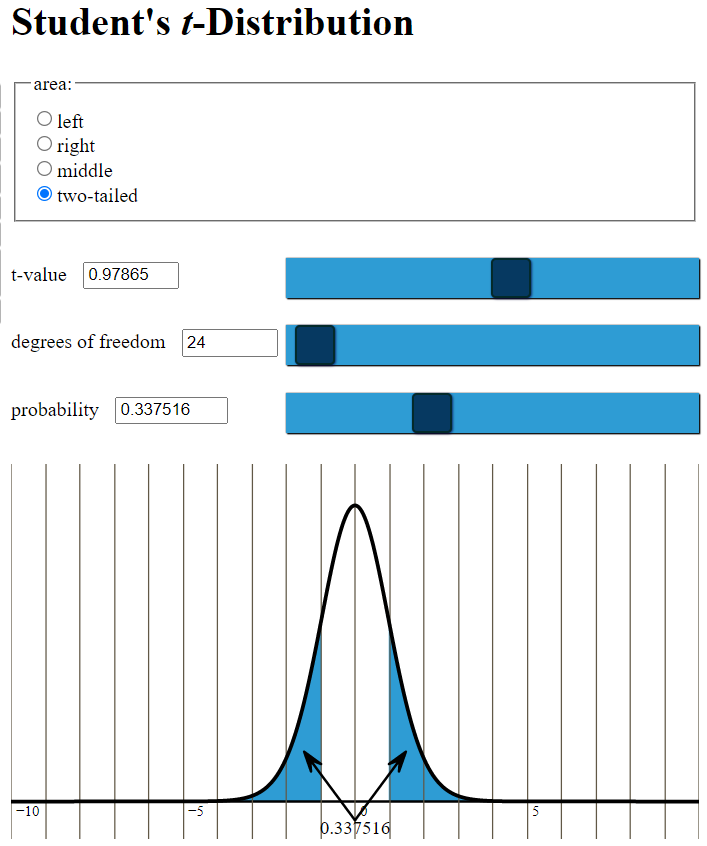
\includegraphics[width=4.5in]{p42.PNG}
            \end{center}

            
    \end{mybox}
\end{enumerate}